% This is the Reed College LaTeX thesis template. Most of the work 
% for the document class was done by Sam Noble (SN), as well as this
% template. Later comments etc. by Ben Salzberg (BTS). Additional
% restructuring and APA support by Jess Youngberg (JY).
% Your comments and suggestions are more than welcome; please email
% them to cus@reed.edu
%
% See http://web.reed.edu/cis/help/latex.html for help. There are a 
% great bunch of help pages there, with notes on
% getting started, bibtex, etc. Go there and read it if you're not
% already familiar with LaTeX.
%
% Any line that starts with a percent symbol is a comment. 
% They won't show up in the document, and are useful for notes 
% to yourself and explaining commands. 
% Commenting also removes a line from the document; 
% very handy for troubleshooting problems. -BTS

% As far as I know, this follows the requirements laid out in 
% the 2002-2003 Senior Handbook. Ask a librarian to check the 
% document before binding. -SN

%%
%% Preamble
%%
% \documentclass{<something>} must begin each LaTeX document
\documentclass[12pt,twoside]{reedthesis}
% Packages are extensions to the basic LaTeX functions. Whatever you
% want to typeset, there is probably a package out there for it.
% Chemistry (chemtex), screenplays, you name it.
% Check out CTAN to see: http://www.ctan.org/
%%
\usepackage{graphicx,latexsym} 
\usepackage{amssymb,amsthm,amsmath}
\usepackage{longtable,booktabs,setspace} 
\usepackage{chemarr} %% Useful for one reaction arrow, useless if you're not a chem major
\usepackage[hyphens]{url}
\usepackage{rotating}
\usepackage{natbib}
\usepackage{listings}
\usepackage{tikz}
\usepackage{algorithm}
\usepackage[noend]{algpseudocode}

% Comment out the natbib line above and uncomment the following two lines to use the new 
% biblatex-chicago style, for Chicago A. Also make some changes at the end where the 
% bibliography is included. 
%\usepackage{biblatex-chicago}
%\bibliography{thesis}

% \usepackage{times} % other fonts are available like times, bookman, charter, palatino

\newcommand{\ceil}[1]{\lceil #1 \rceil}
\newcommand{\floor}[1]{\lfloor #1 \rfloor}

\title{My Final College Paper}
\author{Your R. Name}
% The month and year that you submit your FINAL draft TO THE LIBRARY (May or December)
\date{May 200x}
\division{Mathematics and Natural Sciences}
\advisor{Advisor F. Name}
%If you have two advisors for some reason, you can use the following
%\altadvisor{Your Other Advisor}
%%% Remember to use the correct department!
\department{Mathematics}
% if you're writing a thesis in an interdisciplinary major,
% uncomment the line below and change the text as appropriate.
% check the Senior Handbook if unsure.
%\thedivisionof{The Established Interdisciplinary Committee for}
% if you want the approval page to say "Approved for the Committee",
% uncomment the next line
%\approvedforthe{Committee}

\setlength{\parskip}{0pt}
%%
%% End Preamble
%%
%% The fun begins:
\begin{document}

  \maketitle
  \frontmatter % this stuff will be roman-numbered
  \pagestyle{empty} % this removes page numbers from the frontmatter

% Acknowledgements (Acceptable American spelling) are optional
% So are Acknowledgments (proper English spelling)
    \chapter*{Acknowledgements}
	I want to thank a few people.

% The preface is optional
% To remove it, comment it out or delete it.
    \chapter*{Preface}
	This is an example of a thesis setup to use the reed thesis document class.
	
	

    \chapter*{List of Abbreviations}
		You can always change the way your abbreviations are formatted. Play around with it yourself, use tables, or come to CUS if you'd like to change the way it looks. You can also completely remove this chapter if you have no need for a list of abbreviations. Here is an example of what this could look like:

	\begin{table}[h]
	\centering % You could remove this to move table to the left
	\begin{tabular}{ll}
		\textbf{ABC}  	&  American Broadcasting Company \\
		\textbf{CBS}  	&  Columbia Broadcasting System\\
		\textbf{CDC}  	&  Center for Disease Control \\
		\textbf{CIA}  	&  Central Intelligence Agency\\
		\textbf{CLBR} 	&  Center for Life Beyond Reed\\
		\textbf{CUS}  	&  Computer User Services\\
		\textbf{FBI}  	&  Federal Bureau of Investigation\\
		\textbf{NBC}  	&  National Broadcasting Corporation\\
	\end{tabular}
	\end{table}
	

    \tableofcontents
% if you want a list of tables, optional
    \listoftables
% if you want a list of figures, also optional
    \listoffigures

% The abstract is not required if you're writing a creative thesis (but aren't they all?)
% If your abstract is longer than a page, there may be a formatting issue.
    \chapter*{Abstract}
	The preface pretty much says it all.
	
	\chapter*{Dedication}
	You can have a dedication here if you wish.

  \mainmatter % here the regular arabic numbering starts
  \pagestyle{fancyplain} % turns page numbering back on

%The \introduction command is provided as a convenience.
%if you want special chapter formatting, you'll probably want to avoid using it altogether

% The three lines above are to make sure that the headers are right, that the intro gets included in the table of contents, and that it doesn't get numbered 1 so that chapter one is 1.

% Double spacing: if you want to double space, or one and a half 
% space, uncomment one of the following lines. You can go back to 
% single spacing with the \singlespacing command.
% \onehalfspacing
% \doublespacing


\chapter*{Introduction}
\lstset{language=C++}
\addcontentsline{toc}{chapter}{Introduction}
\chaptermark{Introduction}
\markboth{Introduction}{Introduction}
	
	\section{Overall motivation}
		
		In the heterogeneous computing world, there are tools to create software for specific devices. There are also languages which can compile to many different devices (e.g. OpenCL). However, the number of devices is growing, and their characteristics are getting further apart. There will probably never be one language which works for all devices, and all problems. And there is certainly not one available now. So programmers have to write code for different kinds of devices, so that their application can run efficiently. However, programmers have to rely on their knowledge and intuition to figure out what sorts of hardware is appropriate for their application. As the number of different hardware platforms keeps on growing, this puts more and more strain on software developers to become knowledgeable about all sorts of hardware.
		
		To solve this problem, we suggest making a tool, which can examine CPU code run on a typical workflow, and output suggestions of what kind of hardware different parts of the code can run on. 
		
		This will allow programmers to focus on the hardware platform that is most useful to them reducing search cost. They will still need to learn how to program that hardware, and make their code run efficiently, but at least they will not d all that work to find out that they chose the wrong hardware. 
		
		\subsection{General areas of use cases}
		
		\subsubsection{Performance-Generality tradeoff}
		
		General purpose hardware to improve performance is fairly limited in scope. GPUs are broadly understood by the performance programming community, and more accessible tools are improving at a great pace. FGPAs are quickly catching up. And other coprocessors, like Audio and Encryption accelerators seem to lack proper enough generality to be useful in broad cases [CHECK IF THIS IS ACTUALLY TRUE, LOOK FOR PEOPLE WHO HAVE TRIED TO DO THIS!!!!!!!!!!!!!!!!!!!!!!!!!!!!!].
		
		This is because the tradeoff between generality and performance, which has few points since the software efforts to adopt new hardware is too great to justify too many points.
		
		One possible use case is reducing the cost of adding more points to this curve. If people can match code to hardware capabilities easily, then the search cost of finding the right parts of the software and finding the right parts of the hardware can be reduced. Lowering the cost of changes along this curve can increase granularity, and perhaps bring a new wave of slightly less general hardware. [TALK ABOUT EITAN'S SMART NICs]
		
		However, while this use case is intriguing in theory, in practice, it will change nothing until people are already using it,  which is unlikely if it is not very useful. So we need to look for other useful. 
		
		\subsubsection{Power-Performance tradeoff}
		
		Perhaps the most useful application of this design is helping programmers understand how different hardware platforms will impact power consumption. 
		
		Performance and generality have clear tradeoffs. But when you throw in power into the mix, the hardware world becomes much more daunting.
		
		In power, the hardware can simply adopt similar software interfaces, but have dramatically different 
		
		\footnote{\cite{Taylor:2013}}
		
		There are a wide variety of new hardware 
		
		%\subsection{Mainstream approach}
		
		%Right now, people face the tradeoff between performance and productivity as a fact of life. Except for GPUs, which have mature high level languages, adopting a new hardware platform usually means 
		
		%The reality is that the vast majority of software does not see heterogenous computing as a viable option. Of course, machines are fast enough that we don't have to worry about most software, only ones that consume lots of resources. 
		
		%So what kinds of software are we looking to help?
		
		%The advance of scripting languages such as Python, Ruby, and Javascript means that most modern code is running much slower than it could be if written in a more performance centric language, and so improvements in software can dramatically improve performance and power with no changes to hardware. This is the extreme "productivity" side of the tradeoff,  and there is little we can do here. 
		
		%But the advance of these scripting languages also has brought fast CPU-GPU libraries to exploit various hardware platforms. This is a dominant paradigm in scientific computing. 
		
		%The best supported and most popular libraries, like BLAS, have separate implementations for every imaginable hardware platform. This is the extreme "performance" side of the tradeoff, and again, there is little we can do. 
		
		%\subsection{Best approach (mainstream among theorists)}
		
		%Right now, academics see the most promising route to be changing software models. 
		
		%Existing cross heterogeneous computing languages and paradigms, such as OpenCL, struggle with "performance portability." This means that when the programmer tries to run the code on new hardware, it may run much worse than the original hardware. [CITATION!!!!!!!!!!!!!!!!!!!!!!!!!!!!!]
		
		%\subsection{Improving mainstream approach}
		
		
	\subsection{Note about workload characterization}
		
		A related field of research is workload characterization. The purpose here is to examine how real software runs on hardware, with the purpose of improving the hardware to run the software faster. 
		
		Our work is related since both fields of study are interested in how real software performs on hardware, what sorts of software can run on what sorts of hardware. This means we will use tools originally intended for workload characterization, particularly binary instrumentation tools.
		
		However, the fields have a fundamentally different purpose. We are making a tool to help inform a software developer working with a particular software project about the many different kinds of hardware available. Workload characterization is fundamentally making a tool for the hardware developer, working with a particular piece of hardware, and informing them about the many different types of software. 
		
		This fundamental difference will mean that we cannot copy over the same techniques. In particular, hardware developers have to assume that software runs well “as is” as they cannot hope to improve it. However, software developers can change their software to fit the hardware better. So we need to be much more open to changes in the order of execution of parallel instructions, for example, as they will certainly change when moving from CPU to GPU. 
		
		It seems to me at first glance that this will mean that we need much more complete information about the program than the summary statistics that workload characterization researchers use. 
		
		Two examples I can think of right now are:
		
		\begin{enumerate}
			\item SIMD instruction size: We need to know if the SIMD size expressed by the cpu code is optimal, or if it can be substantially increased by minor changes to the code. This may be the difference of porting it to GPU improving performance or not
			
			\item Level of parallelism. It is kind of difficult to find natural parallelism in arbitrary code to begin with. But when you consider that certain operations (like reductions) are implemented in a highly sequential manner in single threaded programs, but can be rewritten to run in a massively parallel manner. So ideally, we should be able to figure out if they can be written in this way.  (perhaps by keeping track of associative operations)
		\end{enumerate}
		
		\subsection{Note about Intel\textsuperscript{\textregistered} Advisor}
		
		Intel advisor is a very similar tool to what we are using. It's goal is to tell the programmer how they should go about vectorizing and threading their code. This tool can be very effective for both Intel CPUs and Intel Xeon Phi Coprocessors. 
		
		Our end goals are quite separate. Intel's goal is to create an interactive workflow that continuously profiles code on the machine as you optimize it. This is impossible for our purposes, as we will only instrument CPU binary code (this is the only code Intel cares about), and not the code of the machine we are interested in making inferences about.  
		
		But this goal is super important in its own right, and there does not appear to be an open source alternative to intel's tools right now. 
		
		One use case goes like this:
		
		\begin{enumerate}
			\item 
			You are developing code for a system, you profile the code and you find a performance critical section.
			\item You use our tool to understand if this section of code can be parallelized, and what kind of parallelization it can handle (vector, thread, or both). 
			
			\item If the tool tells you it can be parrelelized, and what kind, this will allow you to confidently spend time on this code knowing that it will be worth it. 
			
			If the tool tells you it can't be parrelleized, then it should give you some indication about why it can't be, and where in the code the problem is arising. 
			
			This should allow the programmer to determine if there is some workaround for the problem.
			
			possible problems/fixes:
			
			\begin{enumerate}
				\item Problem: Critical data dependency:
				
				Possible solution: Perhaps there is an algebraic or algorithmic trick that allows you to parrelleize it.
				
				\item Problem: side data dependency (dependency occurs in a logger, assert, or some other non-critical code)
				
				Possible solution: There is usually some workaround here. In the worst case, you can just remove the non-critical code. 
				
				\item Data strides of more than 1 (hurts vectorization):
				
				Possible solution: This can usually be optimized somehow, although sometimes the solution is not trivial. 
				
				\item Non-regular access (vector issues). Similar to previous one, except even less likely to succeed, and even more non-trivial. 
			\end{enumerate}
			
		\end{enumerate} 
		
		Note that while this is useful for developing faster code for a single system, it is also necessary to properly use our tool. Parallelism is a critical input to the analysis, and if it is wrong, because of some minor error that can be fixed easily, then you need to fix it before running the analysis, or else it will make a mistaken analysis. 
		
		And the Intel advisor code involved is very proprietary, and the tools are very expensive (starts at \$1600), and it is not built to be useful for non-Intel processors, or even Intel Integrated Graphics, so it will not be very helpful to achive our goals.
		
		So we need some sort of analysis seperate from Intel Advisor, but which allows for a similar workflow. 
		
	\section{Parts of thesis}
		
		This thesis has several different parts. Although they also build to a single core purpose, they also have other interesting connections, inspirations and applications. 
		
		
		High level implementation description
		
		There will be several parts
		
		Tool which extracts basic runtime information from actual running code (dependencies, memory addresses, instruction type)
		Library which takes basic info from tool and converts it into hardware properties (vector sizes, pipeline sizes, parallelism)
		Library which converts hardware properties into advice about hardware
		
	
	\subsection{Parallelism detection}
		
		\subsubsection{Applications of parallelism detection}
		
		Parallelism detection is super useful for many different applications. 
		
		People have suggested using it for determine where to make speculative automatic parallelization. \footnote{\cite{Chen:2004}} There idea here is that the compiler may not be able to prove that the code is parallel, but it may be able to generate code where if there is not a data conflict, or not many, then there is minimal performance loss. Of course, if there are many dependencies, there may be significant performance loss, so the profiler needs to establish a high degree of parallelism on real inputs. 
		
		It is also useful in a tool which tell the software developer what is parallelizeable and what is not.[CITATION!!!!!!!!!!!!!!!!!!!!!!!!!!!!!!!!!!!!!]
		In larger, complex software, often dependencies are not clearly defined, and manually determining dependencies by sifting through code may be impractical. But dynamic dependency analysis will tell the developer for sure if a block of code can be safely parallelized on the inputs given (it guarantees nothing about other inputs, but this test may be good enough for many developers).
		
		Then, of course, it is critical for our goal. The common theme among new architectures is trading off single threaded performance for power efficiency or high degrees of parallelism [CITATION!!!!!!!!!!!!!!!!!!!!!!!!!!!!!!].
		So determining whether it can exploit parallelism is critical to establishing whether the decrease in sequential performance is will be sufficiently offset by improved parallelism. 
		
		So we need to detect parallelism. How do we go about doing this? (Chapter 1)
		
	\subsection{binary instrumentation}
		\footnote{\cite{Luk:2005}}
		
	\subsection{Hardware identification}
	
	\subsubsection{Things we should consider from software side}
	
	
	\begin{itemize}
		\item Parallelism  (whole section on that)
			\begin{itemize} 
			\item Instruction parallelism (super-scalar vs sequential)
			\item Data parallelism 
			\item Thread parallelism
			\item Reductions
			\end{itemize} 
		
		\item Memory access pattern 
			\begin{itemize} 
			\item is it random
			\item does it allow for vector operations
			\item how many 4k blocks does it touch
			\item Does it stride
			\end{itemize} 
			
		\item Instruction composition
			\begin{itemize} 
			\item Lots of floating points operations?
			\item Complex integer functions (div,mul) vs simple ones (add, lea)?
			\item  
			\end{itemize} 
			
		\item Code pattern
			\begin{itemize} 
			\item Do branches taken in a loop diverge? If so, maybe not GPU, if not, then maybe GPU is good. 
			\item Is there non-trivial recursion or random access code pointers? If so, then many processors like GPUs will not work. 
			\end{itemize} 
		
	\end{itemize}
	
	
	\subsubsection{Things we should consider from hardware side}
	
	\begin{itemize}
		\item Power vs performance need of software (user input)
		
		\item Overhead from shifting between processors:
		
		The big problem is that shifting data across different processors, and telling those processors to do things with that data takes a significant amount of overhead. With GPUs, this can take milliseconds (source). 
		
		\item Superscalar pipelines/dispatch
		
		\item Degree and levels of parallelism in hardware
		
		\item Cache sizes/ hierarchy/ local-shared memory/ 
		
	\end{itemize}

\chapter{Dynamic parallelism detection}
	\section{Data Dependency graphs}
		So how might you detect parallelism? To do that, you have to have a mathematical model of what parallelism is. 
		
		Our model is a dependency graph. 
		
		The idea is that we can take a computation and build a directed acyclic graph like so. There are the input nodes $\{i_1,...,i_n\}$. Each operation is a computation node node in the graph that is pointed to by its inputs. Some of those computation nodes are the outputs. Any node that does not have a path to the outputs is not a valid node. This is a directed acyclic graph because in a computation, no sub-computation can depend on itself. 
		
		For example, you can break the computation of $A+B+D+A\times B$ into a few steps like this
		
		\begin{algorithmic}[1]
			%\Procedure{MyProcedure}{}
			\State $D \gets A+B$
			\State $E \gets A\times B$
			\State $F \gets D+C$
			\State $G \gets E+F$
			%\State $i \gets \textit{patlen}$
			%\If {$i > \textit{stringlen}$} \Return false
			%\EndIf
			%State $j \gets \textit{patlen}$
			%\If {$\textit{string}(i) = \textit{path}(j)$}
			%\State $j \gets j-1$.
			%\State $i \gets i-1$.
			%\State \textbf{goto} \emph{loop}.
			%\State \textbf{close};
			%\EndIf
			%\State $i \gets i+\max(\textit{delta}_1(\textit{string}(i)),\textit{delta}_2(j))$.
			%\State \textbf{goto} \emph{top}.
			%\EndProcedure
		\end{algorithmic}
		
		And then use these sub-operations to build the following dependency graph. 
		
		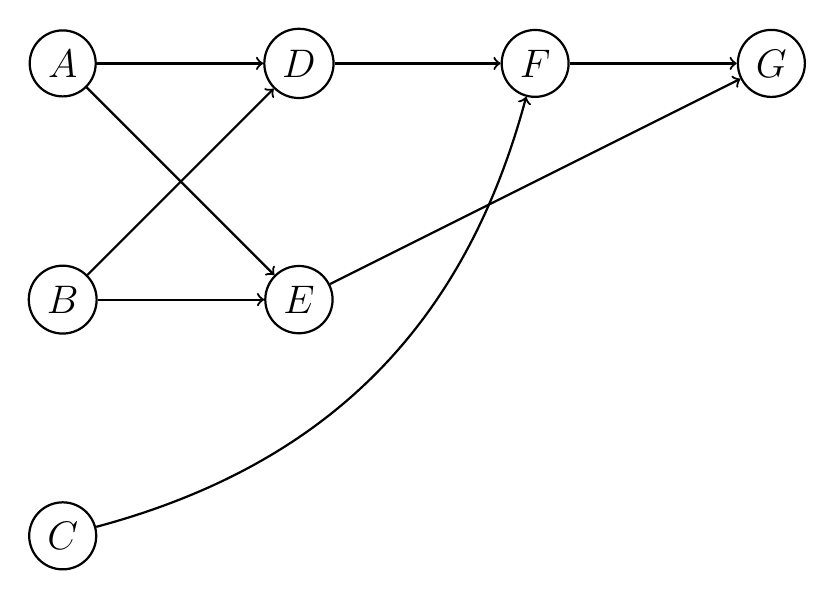
\begin{tikzpicture}[auto, node distance=3cm, every loop/.style={},
		thick,main node/.style={circle,draw,font=\sffamily\Large\bfseries}]
		
		\node[main node] (A) {$A$};
		\node[main node] (B) [below of=A] {$B$};
		\node[main node] (C) [right of=B] {$E$};
		\node[main node] (D) [below of=B] {$C$};
		\node[main node] (F) [right of=A] {$D$};
		\node[main node] (E) [right of=F] {$F$};
		\node[main node] (G) [right of=E] {$G$};
		
		\path[every node/.style={font=\sffamily\small}]
		(A) edge [->] node [left] {} (C)
		(B) edge [->] node [left] {} (C)
		(A) edge [->] node [left] {} (F)
		(B) edge [->] node [left] {} (F)
		(F) edge [->] node [left] {} (E)
		(E) edge [->] node [left] {} (G)
		(C) edge [->] node [left] {} (G)
		(D) [->] edge [bend right] node [left] {} (E);
		\end{tikzpicture}
		%edge [bend right] node[left] {} (2)
		%edge [loop above] node {} (1)
		%(2) edge node [right] {} (1)
		%edge node {} (4)
		%edge [loop left] node {} (2)
		%edge [bend right] node[left] {0.1} (3)
		%(3) edge node [right] {0.8} (2)
		%edge [bend right] node[right] {0.2} (4)
		%(4) edge node [left] {0.2} (3)
		%edge [loop right] node {0.6} (4)
		%edge [bend right] node[right] {0.2} (1);
		
		Hopefully you can see that this is an intuitive framework to examine parrelelizability. In the example above, nodes $D$ and $E$ can be run in parallel since neither depend on the other. $F$ can also be run in parallel with $E$, but not with $D$, since it depends on $D$ already being calculated. $G$ can only be run after all other steps are finished, as it recursively depends on $D,E$, and $F$. 
		
		The degree to which this graph is parallelizable corresponds to the depth of the graph. By depth, we simply mean the maximal length of any path from an input to an output. This can be easily calculated using topological sort. This maximal length is guaranteed to be finite for any directed acyclic graph. In the example above, the depth is 3, as $A\rightarrow D \rightarrow F \rightarrow G$ has 3 edges, and no path has more than 3. 
		
		The most important kind of parallelism, and the only kind we will care about is massive parallelism. Massive parallelism is defined to be any computation where the depth of the dependency graph is logarithmic in the size of the input. 
		
		One extremely simple example of a massively parrellel algorithm is a vector addition. If you want to sum two vectors $a$ and $b$, by computing $c = a+b$, then the obvious algorithm is to take each $i$, and compute $c_i = a_i + b_i$. Since each of these operations is completely dependent on the others, this is a constant depth dependency graph. 
		
		One important example of a massively parrelell algorithm is summing. When you have an array $A_1,A_2,...,A_n$ of numbers and you sum them, there are different ways to do it, some of which are parrelelizable, some of which are not. The most obvious sequential algorithm, computing $(A_1+(A_2+(A_3+...+A_n)))$ has a dependency graph of depth $n$. However, addition is associative, so we can rearrange the parenthesis like this: $(((A_1+A_2)+(A_3+A_4))+...(A_{n-1}+A_n))$ to give us a log depth dependency graph. Below are two algorithms that describe these methods.
		
		\begin{algorithm}
			\caption{MassiveParrelelSum}\label{parellelsum}
			\begin{algorithmic}[1]
				\Function{RecursiveSum}{A,s,e}
					\If {$e - s \le 2$}
						\Return {$\textsc{StandardSum}(A[s:e])$}
					\EndIf
					\State $m \gets \floor{e-s}$
					\State $s_1 \gets \textsc{RecursiveSum}(A,s,m)$
					\State $s_2 \gets \textsc{RecursiveSum}(A,m,e)$
					\State \Return $s_1+s_2$
				\EndFunction
				\Function{StandardSum}{A}
					\State $s \gets 0$
					\For{$a \in A$}
						\State $s \gets s + a$
					\EndFor
				\EndFunction
			\end{algorithmic}
		\end{algorithm}
		
		Now, this is bad since we have two algorithms to compute the same problem, but one of which is parrelizable, and one of which is not. And what allows us to do the transformation from one to the other depends on an algebraic quality that is true for many operations and procedures other than addition. For example subtraction is not associative, but repeated subtraction can have a similar transformation because you can take $\text{RepeatedSubtraction}(A) = -\text{Sum}(A)$, and then do the same log depth calculation with only one more step at the end. 
		
		This general method of using divide and conquer to turn a linear depth operation into a log depth one is called a reduction, and is the basis of the MapReduce cluster computing paradigm. 
		
		Since these are important targets of parallelization, we will try our best to identify these cases, but it is most likely impossible to assess the possibility of this transformation automatically with perfect accuracy, so we will have to analyise actual cases. 
		
		\subsection{Reporting}
		
		Just detecting a binary "is parallel" or "is not parallel" is not particularly useful. If it is a small loop, then it is easy to see if it is parallel or not by hand. A larger loop in real code is quite unlikely to have no data dependencies at all, and so they will rarely be parallel. If the parallelism detector says a larger function is not parallel, then the analysis you do with it won't know if the part that is not parallel is important or not. It could be an assert or logging that is non-vital, or perhaps something that can be pulled out of the loop. However, it is difficult to automatically detect such things, but instead, we can report what in the loop is stopping the function from being parallel to a human. A human, one shown where the problems are, may be able to tell  And a human using this tool won't know where the problem is, and may take a lot of work to find this issues, unless the code tells the human where to look. The most useful information is what instruction the conflicts are coming from, but there are others, for example, the memory location, and the number of accesses which conflict. 
		
		The number of times conflicting accesses happen is useful for us because it gives some indication as to how well it were to perform if we had some sort of locking mechanism serializing accesses to the bit of memory. 
		
		Because this is not the main point of the thesis, I will focus on making a good attempt to report the instruction locations of the conflict, and the number of times conflicts happen. But perfection is not necessary here.
		
		\subsubsection{Reporting List}
		\begin{enumerate}
			\item Whether a loop is parrelell
			\item Number of bytes that conflict between iterations
			\item Instructions that conflicts
			\item etc.
		\end{enumerate}
		
	\section{Pairwise method}
		Note that any naive implementation of actually constructing a data dependence tree from a real computation will take $\Omega(n)$ space, where $n$ is the number of steps of the computation. Even for quick computations, this memory requirement quickly grows beyond RAM capacities of normal machines, and analysis becomes unusably slow. So instead, we will look at special cases and approximations to get what we need. 
	
		The pairwise method is a approximation of data dependence analysis which has been developed to examine loop level parallelism. 
		
		Loop level parallelism is when one iteration of a loop is independent from the rest. This kind of parallelism is the main target of massively parallel architectures. Other types of parallelism, including parallel recursive calls and task parallelism are generally less important or less parrelelizable, than loop level parallelism. 
		
		The idea is to figure out if an iteration of a loop is independent from each other loop iteration. If this is the case, then we have the ability to 
		
		To prove that this always produces a correct answer to the problem, consider the each loop iteration to be a single computation in the graph. The memory addresses that are reads first are clearly inputs to this operation, and the output are writes. 
		
		So if any write of one iteration is read by another, then clearly, this dependency graph is not 1 depth, as the output of one operation is the input of another. 
		
		If the dependency graph is 1, then this means there was no reads of any data that was output in other iterations. 
		
		Note that this being true is critically dependnet on the killed bits operating correcty. After all, in the data dep
		
		%\subsection{Inaccuracy}
		
		%This method is not a perfect calculation of parallelism. Lets look at the following code for a counterexample:
	
%\begin{lstlisting}
%for(int i = 0; i < n; i++){
%	B[i] = A[i-1];
%	A[i] = C[i];
%}
%\end{lstlisting}
		
		%This is clearly parallelizable, yet because the pairwise method focuses on memory locations instead of expressions and calculations, it will determine that this is a read-write dependency, and thus not parallelizable. 
		
		
		
		\subsection{Registers and Flags}
		Unfortunately, memory locations are no the only source of possible memory dependencies. There are also registers.
		
		
		One case of a unparrelelizable register/flag dependency is multiprecision addition.
		
		Say you have 2 numbers of arbitrary size, $A0$, and $B$. $A_i$ is the $i$th 64 bit block of $A$. Then you have the following algorithm to compute addition:
		
		\begin{lstlisting}
cary = 0
for(int i = 0; i < min_size(A,B); i++){
	R[i] = A[i] + B[i] + cary;
	if(overflow_flag){
		cary = 1
	}
	else{
		cary = 0
	}
}
...
		\end{lstlisting}
		
		The first thing to note is that in the worst case, you cannot write to any element of $R_i$ before reading every element of $A$ and $B$ before $i$. So it is not parrelelizable in this case. In practice, it will be somewhat parrelelizable, since that case can safely be assumed to be rare. But a memory-only pairwise method will see that this loop is trivially parrelelizable. On the other hand, looking at the registers, there is a clear read-after-write conflict. 
		
		Some papers ignore this case, as register dependencies can be analyzed statically.\footnote{\cite{Chen:2004}} However,for our uses, we need to know about register dependencies, and so we need to do this either statically or dynamically. 
		
		Static analysis would mean introducing new tools to our project, and even static analysis may yield false negatives of parallelism (due to branching dependences). 
		
		Dynamic analysis of registers could be easily implemented as a special case of memory dependence, as registers can just be considered another type of memory. However, registers are changed far more often than memory, and so we would need to do things somewhat differently if we don't want to suffer a large performance hit. Also, the pairwise method may not be good enough, since 
		
		So we need to make some kind of tradeoff here. I think the right choice is to do dynamic dependence analysis, but keep it quite separate from memory dependence analysis. 
		
		
		\subsubsection{Dependency checking for registers}
		
		Here is an algorithm, assuming we have $n$ registers:
		
		
		
		\subsection{Memory/Performance issues}
		
		Unfortunately, a naive implementation of the pairwise method can consume hundreds of times more memory than the executable code. 
		
		Each loop needs its own copy of all the accesses made by every instruction. This could mean in theory a $cmn$, where $c$ is the number of bytes needed to store the relevant info, (say 20, at least), $m$ is the number of instructions, and $n$ is the number of bytes of memory used by the executable program. 
		
		Of course, in practice it is quite a bit more efficient than this, since not every instruction will access every byte of memory, but it will still take up more memory than most computers can hold just to run basic benchmarks. \footnote{\cite{Kim:2010}}
		
	\section{Stride compression}

		A solution to the memory problems of the pairwise method is stride based compression. The SD3 paper lays this out in some detail \footnote{\cite{Kim:2010}}
		
		\subsection{Goals of compressed algorithm}
		The goal of any compression algorithm of this setting is to compute the things we want to report, without using excessive memory, and without decompression (as this would lead to much slower analysis).
		
		\subsection{SD$^3$ method}
		
		Since both  paper: \footnote{\cite{Kim:2010}}
		
		Doesn’t really work on all code/workloads (need backup system that works decently)
		
		Examples:
		
		Graph computations (simulations, network analysis)
		
		Non-trivial data structures (BST, hash tables)
		
		\subsubsection{More general access compression?}
		
		The innermost loop may not have striding access, but the non-striding access may be similar to its own behavior in a previous iteration of a larger loop (for instance in a graph computation where it iterates over all the edges of a vertex in each iteration of a loop). 
		
		
		Idea: We can see all accesses of data as the set of permutations of memory addresses. We know that there are patterns in accesses. We can make a general purpose compression of memory accesses, where the stride compression is a special case of. 
		
		Trick: We need to somehow do efficient computations on these things.
		
		
		\subsection{Dependency collision function}
		
		\subsection{Kill bit collision function}
		
		\subsection{Bit calculation performance optimization}
		
		
		
	\section{Stride compression}
		
		\subsection{Examples of different kinds of strides}
		The most common and important kind of stride is accessing every element of standard array. This can be a dense stride, if you are accessing the entire element. But often, you have a array of structs, and you are only accessing part of the struct in the loop. This is a $ $
		
		The other main kind is going along an axis of an $n$-dimensional grid. 
		
		But there are other kinds of stride accesses. For instance: diagonals on an $n$-dimensional grid (bishop movement in chess). Or linear derandomization, like in linear open hashing. 
		
	\section{Stride based dependency checking on normal access patterns}
		
		Lets say we have 2 strides in the form $[ax+c]$ for $0\le x \le \alpha$, and $[by+d]$, for $0 \le y \le \beta$. We want to quickly and efficiently check if there is a dependency, and if so, then where they are. 
		
		GCD negative check: If $|d-c| \ne 0 \mod \gcd(a,b)$, then there is no dependency. Intuitively, this is true because if the difference between the strides is a value that cannot be taken by combinations of $a$ and $b$, then there can never be an overlap. 
		
		Interval Overlap Check: If intervals $[c,a\alpha+c]$, $[d,d+b\beta]$ do not overlap, then there is no dependency. 
		
		In order to have a positive check for dependencies, and to count the number of dependencies, there is a little more you have to do, but it can still be done efficiently. 
		
		\subsection{Handling different sized blocks}
		
		Unfortunately, things are more complicated then they might seem just looking at the above. 
		The reason is that hardware allows memory accesses of varying bytes on the same data. For example, you might examine a text one byte at a time, and then later examine it in 8 byte blocks. Even worse, common hardware does not force aligned access. So there might be a 4 byte access with stride length of 12 bytes, starting from 3, and a 8 byte access of 16 stride length starting from 7. So we need to introduce another concept to stride checking in order to make this work: block size. 
		
		There is an efficient way of finding if there is an dependency, assuming strides length is a multiple of block size for all strides. And we can just make our stride detector only detect strides like this.
		
		But how do we find the exact number of dependencies and where they are? What do we do about killed bits in this context (since this can lead to really awkward strides)? 
		
		So instead of carefully dealing with abnormal strides like this slowly and carefully, I will instead just make basic checks, and then assume the worst case, whatever that may be in this context. 

\chapter{The First}
  	This is the first page of the first chapter. You may delete the contents of this chapter so you can add your own text; it's just here to show you some examples. 
	
	\section{References, Labels, Custom Commands and Footnotes}
	It is easy to refer to anything within your document using the \texttt{label} and \texttt{ref} tags.  Labels must be unique and shouldn't use any odd characters; generally sticking to letters and numbers (no spaces) should be fine. Put the label on whatever you want to refer to, and put the reference where you want the reference. \LaTeX\ will keep track of the chapter, section, and figure or table numbers for you. 
	
	\subsection{References and Labels}
	Sometimes you'd like to refer to a table or figure, e.g. you can see in Figure \ref{subd2} that you can rotate figures . Start by labeling your figure or table with the label command (\verb=\label{labelvariable}=) below the caption (see the chapter on graphics and tables for examples). Then when you would like to refer to the table or figure, use the ref command (\verb=\ref{labelvariable}=). Make sure your label variables are unique; you can't have two elements named ``default." Also, since the reference command only puts the figure or table number, you will have to put  ``Table" or ``Figure" as appropriate, as seen in the following examples:
	
	 As I showed in Table \ref{inheritance} many factors can be assumed to follow from inheritance. Also see the Figure \ref{subd} for an illustration.
		 
	\subsection{Custom Commands}\label{commands}
	Are you sick of writing the same complex equation or phrase over and over? 
	
	The custom commands should be placed in the preamble, or at least prior to the first usage of the command. The structure of the \verb=\newcommand= consists of the name of the new command in curly braces, the number of arguments to be made in square brackets and then, inside a new set of curly braces, the command(s) that make up the new command. The whole thing is sandwiched inside a larger set of curly braces. 
	
	% Note: you cannot use numbers in your commands!
	\newcommand{\hydro}{H$_2$SO$_4$}
	
	In other words, if you want to make a shorthand for H$_2$SO$_4$, which doesn't include an argument, you would write: \verb=\newcommand{\hydro}{H$_2$SO$_4$}= and then when you needed  to use the command you would type \verb=\hydro=. (sans verb and the equals sign brackets, if you're looking at the .tex version). For example: \hydro

	\subsection{Footnotes and Endnotes}
		You might want to footnote something.\footnote{footnote text} Be sure to leave no spaces between the word immediately preceding the footnote command and the command itself. The footnote will be in a smaller font and placed appropriately. Endnotes work in much the same way. More information can be found about both on the CUS site.
		
	\section{Bibliographies}
		Of course you will need to cite things, and you will probably accumulate an armful of sources. This is why BibTeX was created. For more information about BibTeX and bibliographies, see our CUS site (\url{web.reed.edu/cis/help/latex/index.html})\footnote{\cite{reedweb:2007}}. There are three pages on this topic: {\it bibtex} (which talks about using BibTeX, at \url{/latex/bibtex.html}), {\it bibtexstyles} (about how to find and use the bibliography style that best suits your needs, at \url{/latex/bibtexstyles.html}) and {\it bibman} (which covers how to make and maintain a bibliography by hand, without BibTeX, at at \url{/latex/bibman.html}). The last page will not be useful unless you have only a few sources. There used to be APA stuff here, but we don't need it since I've fixed this with my apa-good natbib style file.
		
	\subsection{Tips for Bibliographies}
	\begin{enumerate}
	\item Like with thesis formatting, the sooner you start compiling your bibliography for something as large as thesis, the better. Typing in source after source is mind-numbing enough; do you really want to do it for hours on end in late April? Think of it as procrastination.
	\item The cite key (a citation's label) needs to be unique from the other entries.
	\item When you have more than one author or editor, you need to separate each author's name by the word ``and'' e.g.\\ \verb+Author = {Noble, Sam and Youngberg, Jessica},+.
	\item Bibliographies made using BibTeX (whether manually or using a manager) accept LaTeX markup, so you can italicize and add symbols as necessary.
	\item To force capitalization in an article title or where all lowercase is generally used, bracket the capital letter in curly braces.
	\item You can add a Reed Thesis citation\footnote{\cite{noble:2002}} option. The best way to do this is to use the phdthesis type of citation, and use the optional ``type'' field to enter ``Reed thesis'' or ``Undergraduate thesis''. Here's a test of Chicago, showing the second cite in a row\footnote{\cite{noble:2002}} being different. Also the second time not in a row\footnote{\cite{reedweb:2007}} should be different. Of course in other styles they'll all look the same.
	\end{enumerate}
	\section{Anything else?}
	If you'd like to see examples of other things in this template, please contact CUS (email cus@reed.edu) with your suggestions. We love to see people using \LaTeX\ for their theses, and are happy to help.


\chapter{Mathematics and Science}	
	\section{Math}
		\TeX\ is the best way to typeset mathematics. Donald Knuth designed \TeX\ when he got frustrated at how long it was taking the typesetters to finish his book, which contained a lot of mathematics. 
		
		If you are doing a thesis that will involve lots of math, you will want to read the following section which has been commented out. If you're not going to use math, skip over this next big red section. (It's red in the .tex file but does not show up in the .pdf.)
	
% MATH and PHYSICS majors: Uncomment the following section	
	$$\sum_{j=1}^n (\delta\theta_j)^2 \leq {{\beta_i^2}\over{\delta_i^2 + \rho_i^2}}
\left[ 2\rho_i^2 + {\delta_i^2\beta_i^2\over{\delta_i^2 + \rho_i^2}} \right] \equiv \omega_i^2
$$

From Informational Dynamics, we have the following (Dave Braden):

After {\it n} such encounters the posterior density for $\theta$ is

$$
\pi(\theta|X_1< y_1,\dots,X_n<y_n) \varpropto \pi(\theta) \prod_{i=1}^n\int_{-\infty}^{y_i}
   \exp\left(-{(x-\theta)^2\over{2\sigma^2}}\right)\ dx
$$



Another equation:

$$\det\left|\,\begin{matrix}%
c_0&c_1\hfill&c_2\hfill&\ldots&c_n\hfill\cr
c_1&c_2\hfill&c_3\hfill&\ldots&c_{n+1}\hfill\cr
c_2&c_3\hfill&c_4\hfill&\ldots&c_{n+2}\hfill\cr
\,\vdots\hfill&\,\vdots\hfill&
  \,\vdots\hfill&&\,\vdots\hfill\cr
c_n&c_{n+1}\hfill&c_{n+2}\hfill&\ldots&c_{2n}\hfill\cr
\end{matrix}\right|>0$$


Lapidus and Pindar, Numerical Solution of Partial Differential Equations in Science and
Engineering.  Page 54

$$
\int_t\left\{\sum_{j=1}^3 T_j \left({d\phi_j\over dt}+k\phi_j\right)-kT_e\right\}w_i(t)\ dt=0,
   \qquad\quad i=1,2,3. 
$$

L\&P  Galerkin method weighting functions.  Page 55

$$
\sum_{j=1}^3 T_j\int_0^1\left\{{d\phi_j\over dt} + k\phi_j\right\} \phi_i\ dt 
   = \int_{0}^1k\,T_e\phi_idt, \qquad i=1,2,3 $$
   
Another L\&P (p145)

$$
\int_{-1}^1\!\int_{-1}^1\!\int_{-1}^1 f\big(\xi,\eta,\zeta\big) 
   = \sum_{k=1}^n\sum_{j=1}^n\sum_{i=1}^n w_i w_j w_k f\big( \xi,\eta,\zeta\big).
$$

Another L\&P (p126)

$$
\int_{A_e} (\,\cdot\,) dx dy = \int_{-1}^1\!\int_{-1}^1 (\,\cdot\,) \det[J] d\xi d\eta.
$$

\section{Chemistry 101: Symbols}
Chemical formulas will look best if they are not italicized. Get around math mode's automatic italicizing by using the argument \verb=$\mathrm{formula here}$=, with your formula inside the curly brackets.

So, $\mathrm{Fe_2^{2+}Cr_2O_4}$ is written \verb=$\mathrm{Fe_2^{2+}Cr_2O_4}$=\\
Exponent or Superscript: O$^{-}$\\
Subscript: CH$_{4}$\\

To stack numbers or letters as in $\mathrm{Fe_2^{2+}}$, the subscript is defined first, and then the superscript is defined.\\
Angstrom: {\AA}\\
Bullet: CuCl $\bullet$ 7H${_2}$O\\
Double Dagger: \ddag \/\\
Delta: $\Delta$\\
Reaction Arrows: $\longrightarrow$ or  $\xrightarrow{solution}$\\
Resonance Arrows: $\leftrightarrow$\\
Reversible Reaction Arrows: $\rightleftharpoons$ or $\xrightleftharpoons[ ]{solution}$ (the latter requires the chemarr package)\\


\subsection{Typesetting reactions}
You may wish to put your reaction in a figure environment, which means that LaTeX will place the reaction where it fits and you can have a figure legend if desired:
\begin{figure}[htbp]
\begin{center}
$\mathrm{C_6H_{12}O_6  + 6O_2} \longrightarrow \mathrm{6CO_2 + 6H_2O}$
\caption{Combustion of glucose}
\label{combustion of glucose}
\end{center}
\end{figure}

\subsection{Other examples of reactions}
$\mathrm{NH_4Cl_{(s)}} \rightleftharpoons \mathrm{NH_{3(g)}+HCl_{(g)}}$\\
$\mathrm{MeCH_2Br + Mg} \xrightarrow[below]{above} \mathrm{MeCH_2\bullet Mg \bullet Br}$

\section{Physics}

Many of the symbols you will need can be found on the math page (\url{http://web.reed.edu/cis/help/latex/math.html}) and the Comprehensive \LaTeX\ Symbol Guide (enclosed in this template download).  You may wish to create custom commands for commonly used symbols, phrases or equations, as described in Chapter \ref{commands}.

\section{Biology}
You will probably find the resources at \url{http://www.lecb.ncifcrf.gov/~toms/latex.html} helpful, particularly the links to bsts for various journals. You may also be interested in TeXShade for nucleotide typesetting (\url{http://homepages.uni-tuebingen.de/beitz/txe.html}).  Be sure to read the proceeding chapter on graphics and tables, and remember that the thesis template has versions of Ecology and Science bsts which support webpage citation formats. 

\chapter{Tables and Graphics}

\section{Tables}
	The following section contains examples of tables, most of which have been commented out for brevity. (They will show up in the .tex document in red, but not at all in the .pdf). For more help in constructing a table (or anything else in this document), please see the LaTeX pages on the CUS site. 

\begin{table}[htbp] % begins the table floating environment. This enables LaTeX to fit the table where it works best and lets you add a caption.
\caption[Correlation of Inheritance Factors between Parents and Child]{Correlation of Inheritance Factors between Parents and Child} 
% The words in square brackets of the caption command end up in the Table of Tables. The words in curly braces are the caption directly over the table.
\begin{center} 
% makes the table centered
\begin{tabular}{c c c c} 
% the tabular environment is used to make the table itself. The {c c c c} specify that the table will have four columns and they will all be center-aligned. You can make the cell contents left aligned by replacing the Cs with Ls or right aligned by using Rs instead. Add more letters for more columns, and pipes (the vertical line above the backslash) for vertical lines. Another useful type of column is the p{width} column, which forces text to wrap within whatever width you specify e.g. p{1in}. Text will wrap badly in narrow columns though, so beware.
\toprule % a horizontal line, slightly thicker than \hline, depends on the booktabs package
  Factors &  Correlation between Parents \& Child & Inherited \\ % the first row of the table. Separate columns with ampersands and end the line with two backslashes. An environment begun in one cell will not carry over to adjacent rows.
  \midrule % another horizontal line
	Education 				& -0.49 & Yes 	 \\ % another row
	Socio-Economic Status 	& 0.28 	& Slight \\
	Income 					& 0.08 	& No	 \\
	Family Size 			& 0.19 	& Slight \\
	Occupational Prestige 	& 0.21 	& Slight \\
\bottomrule % yet another horizontal line
\end{tabular}
\end{center}
\label{inheritance} % labels are useful when you have more than one table or figure in your document. See our online documentation for more on this.
\end{table}

	\clearpage 
%% \clearpage ends the page, and also dumps out all floats. 
%% Floats are things like tables and figures.

If you want to make a table that is longer than a page, you will want to use the longtable environment. Uncomment the table below to see an example, or see our online documentation.

%% An example of a long table, with headers that repeat on each subsequent page: Results from the summers of 1998 and 1999 work at Reed College done by Grace Brannigan, Robert Holiday and Lien Ngo in 1998 and Kate Brown and Christina Inman in 1999.

	\begin{longtable}{||c|c|c|c||}
	 	\caption[Chromium Hexacarbonyl Data Collected in 1998--1999]{Chromium Hexacarbonyl Data Collected in 1998--1999}\\ \hline
	    	  \multicolumn{4}{||c||}{Chromium Hexacarbonyl} \\\hline
		   State & Laser wavelength & Buffer gas & Ratio of $\frac{\textrm{Intensity
at vapor pressure}}{\textrm{Intensity at 240 Torr}}$ \\ \hline
		  \endfirsthead
		\hline     State & Laser wavelength & Buffer gas & Ratio of
$\frac{\textrm{Intensity at vapor pressure}}{\textrm{Intensity at 240 Torr}}$\\
\hline
		    \endhead

	    $z^{7}P^{\circ}_{4}$ & 266 nm & Argon & 1.5 \\\hline
	    $z^{7}P^{\circ}_{2}$ & 355 nm & Argon & 0.57 \\\hline
	    $y^{7}P^{\circ}_{3}$ & 266 nm & Argon & 1 \\\hline
	    $y^{7}P^{\circ}_{3}$ & 355 nm & Argon & 0.14 \\\hline
	    $y^{7}P^{\circ}_{2}$ & 355 nm & Argon & 0.14 \\\hline
	    $z^{5}P^{\circ}_{3}$ & 266 nm & Argon & 1.2 \\\hline
	    $z^{5}P^{\circ}_{3}$ & 355 nm & Argon & 0.04 \\\hline
	    $z^{5}P^{\circ}_{3}$ & 355 nm & Helium & 0.02 \\\hline
	    $z^{5}P^{\circ}_{2}$ & 355 nm & Argon & 0.07 \\\hline
	    $z^{5}P^{\circ}_{1}$ & 355 nm & Argon & 0.05 \\\hline
	    $y^{5}P^{\circ}_{3}$ & 355 nm & Argon & 0.05, 0.4 \\\hline
	    $y^{5}P^{\circ}_{3}$ & 355 nm & Helium & 0.25 \\\hline
	    $z^{5}F^{\circ}_{4}$ & 266 nm & Argon & 1.4 \\\hline
	    $z^{5}F^{\circ}_{4}$ & 355 nm & Argon & 0.29 \\\hline
	    $z^{5}F^{\circ}_{4}$ & 355 nm & Helium & 1.02 \\\hline
	    $z^{5}D^{\circ}_{4}$ & 355 nm & Argon & 0.3 \\\hline
	    $z^{5}D^{\circ}_{4}$ & 355 nm & Helium & 0.65 \\\hline
	    $y^{5}H^{\circ}_{7}$ & 266 nm & Argon & 0.17 \\\hline
	    $y^{5}H^{\circ}_{7}$ & 355 nm & Argon & 0.13 \\\hline
	    $y^{5}H^{\circ}_{7}$ & 355 nm & Helium & 0.11 \\\hline
	    $a^{5}D_{3}$ & 266 nm & Argon & 0.71 \\\hline
	    $a^{5}D_{2}$ & 266 nm & Argon & 0.77 \\\hline
	    $a^{5}D_{2}$ & 355 nm & Argon & 0.63 \\\hline
	    $a^{3}D_{3}$ & 355 nm & Argon & 0.05 \\\hline
	    $a^{5}S_{2}$ & 266 nm & Argon & 2 \\\hline
	    $a^{5}S_{2}$ & 355 nm & Argon & 1.5 \\\hline
	    $a^{5}G_{6}$ & 355 nm & Argon & 0.91 \\\hline
	    $a^{3}G_{4}$ & 355 nm & Argon & 0.08 \\\hline
	    $e^{7}D_{5}$ & 355 nm & Helium & 3.5 \\\hline
	    $e^{7}D_{3}$ & 355 nm & Helium & 3 \\\hline
	    $f^{7}D_{5}$ & 355 nm & Helium & 0.25 \\\hline
	    $f^{7}D_{5}$ & 355 nm & Argon & 0.25 \\\hline
	    $f^{7}D_{4}$ & 355 nm & Argon & 0.2 \\\hline
	    $f^{7}D_{4}$ & 355 nm & Helium & 0.3 \\\hline
	    \multicolumn{4}{||c||}{Propyl-ACT} \\\hline
%	    State & Laser wavelength & Buffer gas & Ratio of $\frac{\textrm{Intensity
%at vapor pressure}}{\textrm{Intensity at 240 Torr}}$\\ \hline
	    $z^{7}P^{\circ}_{4}$ & 355 nm & Argon & 1.5 \\\hline
	    $z^{7}P^{\circ}_{3}$ & 355 nm & Argon & 1.5 \\\hline
	    $z^{7}P^{\circ}_{2}$ & 355 nm & Argon & 1.25 \\\hline
	    $z^{7}F^{\circ}_{5}$ & 355 nm & Argon & 2.85 \\\hline
	    $y^{7}P^{\circ}_{4}$ & 355 nm & Argon & 0.07 \\\hline
	    $y^{7}P^{\circ}_{3}$ & 355 nm & Argon & 0.06 \\\hline
	    $z^{5}P^{\circ}_{3}$ & 355 nm & Argon & 0.12 \\\hline
	    $z^{5}P^{\circ}_{2}$ & 355 nm & Argon & 0.13 \\\hline
	    $z^{5}P^{\circ}_{1}$ & 355 nm & Argon & 0.14 \\\hline
	    \multicolumn{4}{||c||}{Methyl-ACT} \\\hline
%	    State & Laser wavelength & Buffer gas & Ratio of $\frac{\textrm{Intensity
% at vapor pressure}}{\textrm{Intensity at 240 Torr}}$\\ \hline
	    $z^{7}P^{\circ}_{4}$ & 355 nm & Argon & 1.6, 2.5 \\\hline
	    $z^{7}P^{\circ}_{4}$ & 355 nm & Helium & 3 \\\hline
	    $z^{7}P^{\circ}_{4}$ & 266 nm & Argon & 1.33 \\\hline
	    $z^{7}P^{\circ}_{3}$ & 355 nm & Argon & 1.5 \\\hline
	    $z^{7}P^{\circ}_{2}$ & 355 nm & Argon & 1.25, 1.3 \\\hline
	    $z^{7}F^{\circ}_{5}$ & 355 nm & Argon & 3 \\\hline
	    $y^{7}P^{\circ}_{4}$ & 355 nm & Argon & 0.07, 0.08 \\\hline
	    $y^{7}P^{\circ}_{4}$ & 355 nm & Helium & 0.2 \\\hline
	    $y^{7}P^{\circ}_{3}$ & 266 nm & Argon & 1.22 \\\hline
	    $y^{7}P^{\circ}_{3}$ & 355 nm & Argon & 0.08 \\\hline
	    $y^{7}P^{\circ}_{2}$ & 355 nm & Argon & 0.1 \\\hline
	    $z^{5}P^{\circ}_{3}$ & 266 nm & Argon & 0.67 \\\hline
	    $z^{5}P^{\circ}_{3}$ & 355 nm & Argon & 0.08, 0.17 \\\hline
	    $z^{5}P^{\circ}_{3}$ & 355 nm & Helium & 0.12 \\\hline
	    $z^{5}P^{\circ}_{2}$ & 355 nm & Argon & 0.13 \\\hline
	    $z^{5}P^{\circ}_{1}$ & 355 nm & Argon & 0.09 \\\hline
	    $y^{5}H^{\circ}_{7}$ & 355 nm & Argon & 0.06, 0.05 \\\hline
	    $a^{5}D_{3}$ & 266 nm & Argon & 2.5 \\\hline
	    $a^{5}D_{2}$ & 266 nm & Argon & 1.9 \\\hline
	    $a^{5}D_{2}$ & 355 nm & Argon & 1.17 \\\hline
	    $a^{5}S_{2}$ & 266 nm & Argon & 2.3 \\\hline
	    $a^{5}S_{2}$ & 355 nm & Argon & 1.11 \\\hline
	    $a^{5}G_{6}$ & 355 nm & Argon & 1.6 \\\hline
	    $e^{7}D_{5}$ & 355 nm & Argon & 1 \\\hline

		\end{longtable}

   
   \section{Figures}
   
	If your thesis has a lot of figures, \LaTeX\ might behave better for you than that other word processor.  One thing that may be annoying is the way it handles ``floats'' like tables and figures. \LaTeX\ will try to find the best place to put your object based on the text around it and until you're really, truly done writing you should just leave it where it lies.   There are some optional arguments to the figure and table environments to specify where you want it to appear; see the comments in the first figure.

	If you need a graphic or tabular material to be part of the text, you can just put it inline. If you need it to appear in the list of figures or tables, it should be placed in the floating environment. 
	
	To get a figure from StatView, JMP, SPSS or other statistics program into a figure, you can print to pdf or save the image as a jpg or png. Precisely how you will do this depends on the program: you may need to copy-paste figures into Photoshop or other graphic program, then save in the appropriate format.
	
	Below we have put a few examples of figures. For more help using graphics and the float environment, see our online documentation.
	
	And this is how you add a figure with a graphic:
	\begin{figure}[h]
	% the options are h = here, t = top, b = bottom, p = page of figures.
	% you can add an exclamation mark to make it try harder, and multiple
	% options if you have an order of preference, e.g.
	% \begin{figure}[h!tbp]
	   
	       \centering
	    % DO NOT ADD A FILENAME EXTENSION TO THE GRAPHIC FILE
	    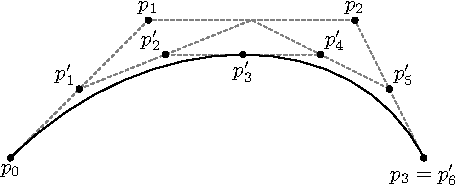
\includegraphics{subdivision}
	     \caption{A Figure}
	 \label{subd}
	\end{figure}

\clearpage %% starts a new page and stops trying to place floats such as tables and figures

\section{More Figure Stuff}
You can also scale and rotate figures.
 	\begin{figure}[h!]
	   
	       \centering
	    % DO NOT ADD A FILENAME EXTENSION TO THE GRAPHIC FILE
	    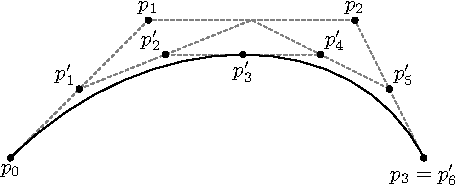
\includegraphics[scale=0.5,angle=180]{subdivision}
	    % if your figure shows up not where you want it, it may just be too big to fit. You can use the scale argument to shrink it, e.g. scale=0.85 is 85 percent of the original size. 
	     \caption{A Smaller Figure, Flipped Upside Down}
	 \label{subd2}
	\end{figure}

\section{Even More Figure Stuff}
With some clever work you can crop a figure, which is handy if (for instance) your EPS or PDF is a little graphic on a whole sheet of paper. The viewport arguments are the lower-left and upper-right coordinates for the area you want to crop.

 	\begin{figure}[h!]
	    	       \centering
	    % DO NOT ADD A FILENAME EXTENSION TO THE GRAPHIC FILE
	   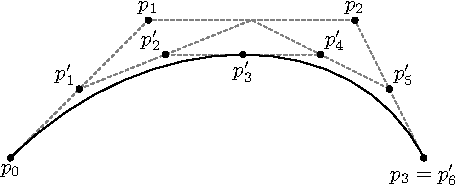
\includegraphics[clip=true, viewport=.0in .0in 1in 1in]{subdivision}
	    \caption{A Cropped Figure}
	 \label{subd3}
	\end{figure}
	
      \subsection{Common Modifications}
      The following figure features the more popular changes thesis students want to their figures. This information is also on the web at \url{web.reed.edu/cis/help/latex/graphics.html}.
    %\renewcommand{\thefigure}{0.\arabic{figure}} 	% Renumbers the figure to the type 0.x
    %\addtocounter{figure}{4} 						% starts the figure numbering at 4
    \begin{figure}[htbp]
    \begin{center}
   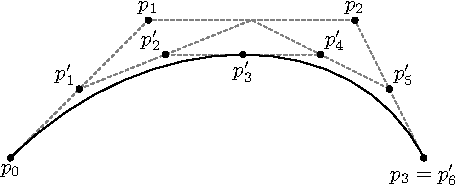
\includegraphics[scale=0.5]{subdivision}
    \caption[Subdivision of arc segments]{\footnotesize{Subdivision of arc segments. You can see that $ p_3 = p_6^\prime$.}} %the special ToC caption is in square brackets. The \footnotesize makes the figure caption smaller
    \label{barplot}
    \end{center}
    \end{figure} 

\chapter*{Conclusion}
         \addcontentsline{toc}{chapter}{Conclusion}
	\chaptermark{Conclusion}
	\markboth{Conclusion}{Conclusion}
	\setcounter{chapter}{4}
	\setcounter{section}{0}
	
Here's a conclusion, demonstrating the use of all that manual incrementing and table of contents adding that has to happen if you use the starred form of the chapter command. The deal is, the chapter command in \LaTeX\ does a lot of things: it increments the chapter counter, it resets the section counter to zero, it puts the name of the chapter into the table of contents and the running headers, and probably some other stuff. 

So, if you remove all that stuff because you don't like it to say ``Chapter 4: Conclusion'', then you have to manually add all the things \LaTeX\ would normally do for you. Maybe someday we'll write a new chapter macro that doesn't add ``Chapter X'' to the beginning of every chapter title.

\section{More info}
And here's some other random info: the first paragraph after a chapter title or section head \emph{shouldn't be} indented, because indents are to tell the reader that you're starting a new paragraph. Since that's obvious after a chapter or section title, proper typesetting doesn't add an indent there. 


%If you feel it necessary to include an appendix, it goes here.
    \appendix
      \chapter{The First Appendix}
      \chapter{The Second Appendix, for Fun}


%This is where endnotes are supposed to go, if you have them.
%I have no idea how endnotes work with LaTeX.

  \backmatter % backmatter makes the index and bibliography appear properly in the t.o.c...

% if you're using bibtex, the next line forces every entry in the bibtex file to be included
% in your bibliography, regardless of whether or not you've cited it in the thesis.
    \nocite{*}

% Rename my bibliography to be called "Works Cited" and not "References" or ``Bibliography''
% \renewcommand{\bibname}{Works Cited}

%    \bibliographystyle{bsts/mla-good} % there are a variety of styles available; 
%  \bibliographystyle{plainnat}
% replace ``plainnat'' with the style of choice. You can refer to files in the bsts or APA 
% subfolder, e.g. 
 \bibliographystyle{APA/apa-good}  % or
 \bibliography{thesis}
 % Comment the above two lines and uncomment the next line to use biblatex-chicago.
 %\printbibliography[heading=bibintoc]

% Finally, an index would go here... but it is also optional.
\end{document}
